\subsection{Implementation Verification}\label{plan:implementation}
The goal of implementation verification is to evaluate \progname{}'s source
code and its documentation for correctness, consistency, completeness,
accuracy, readability, testability, and traceability. This corresponds to the
source code and source code documentation evaluation and traceability analysis
tasks in Section 9.4 of IEEE Std 1012-2016~\citep{vvIEEE}.

\paragraph{Method} The implementation verification plan uses both static and
dynamic testing methods:
\begin{enumerate}

    \item Static Testing Method \\
    The source code and its documentation is statically tested by peer review.
    A peer review tests: the source code for traceability to Module Interface
    Specification (MIS) document and consistent use of coding standards and
    quality; and the source code's documentation for correctness, completeness,
    consistency, and readability.

    The peer review has the following stages:
    \begin{enumerate}

        \item Preparation: Participants review the source code and its
        documentation with respect to their assigned role and goals
        (Table~\ref{tab:rolesImplementation})

        \item Meeting: Participants meet to discuss findings, potential issues,
        and proposed action plans to address them

        \item Rework: The source code/documentation author revises the
        code/documentation to address raised issues, guided by the proposed
        action plans

        \item Follow Up: Participants verify that raised issues have been
        addressed satisfactorily

    \end{enumerate}

    A recording device might be used to capture meeting proceedings in place of
    physical note taking so that all participants can focus on the discussion.

    Peer review begins when there is a new major version of the source code
    and/or its documentation.

    Peer review ends when reviewers agree that there are no issues that will
    likely result in an extensive loss of confidence in \progname{} (e.g.
    inconsistent naming conventions).

    \item Dynamic Testing Method \\
    Test cases dynamically test the source code for its adherence to the
    behaviours specified in the functional requirements in the Software
    Requirements Specification (SRS) and the characteristics and/or properties
    specified in the nonfunctional requirements in the SRS.

    For information about test case types, specifications, and traceability to
    \progname{}'s requirements, see the ``System, Integration, and Unit Test
    Plan for \progname{}: A Computational Model of Emotion for Enhancing
    Non-Player Character Believability in Games'' document.

\end{enumerate}

%Dynamic methods:
%\begin{itemize}
%
%    \item Boundary testing
%
%    \item Default/Null testing
%
%    \item Garbage data testing
%
%    \item State testing
%
%    \item Race condition testing
%
%    \item Repetition, Stress, and Load testing
%
%    \item Code coverage testing
%
%\end{itemize}

\paragraph{Roles and Responsibilities} To assist in the achievement of their
assigned goals (Table~\ref{tab:rolesImplementation}):
\begin{enumerate}

    \item Static Testing
    \begin{itemize}

        \item Primary team members are responsible for ensuring that reviewers
        have the necessary materials, moderating the peer review process and
        reading through the document(s) during the meeting(s)

        \item Secondary and tertiary members are reviewers whom are responsible
        for reviewing the source code and source code documentation prior to
        the meeting so that they are prepared to discuss it with the team

    \end{itemize}

    \item Dynamic Testing
    \begin{itemize}

        \item Primary team members are responsible for generating and
        implementing test cases and automated tools as described in the
        ``System, Integration, and Unit Test Plan for \progname{}: A
        Computational Model of Emotion for Enhancing Non-Player Character
        Believability in Games'' document

        \item Secondary and tertiary members do not participate in dynamic
        testing

    \end{itemize}

\end{enumerate}

\paragraph{Inputs}
\begin{itemize}

    \item Source Code and Documentation for \progname{}: A Computational Model
    of Emotion for Enhancing Non-Player Character Believability in Games

    \item Module Guide for \progname{}: A Computational Model of Emotion for
    Enhancing Non-Player Character Believability in Games

    \item Module Interface Specification for \progname{}: A Computational Model
    of Emotion for Enhancing Non-Player Character Believability in Games

    \item Coding standards for the source code's implementation language

    \item Review guide for \progname{}'s source code and its documentation
    (Appendix~\ref{appendix:verificationInspection})

    \item System, Integration, and Unit Test Plan for \progname{}: A
    Computational Model of Emotion for Enhancing Non-Player Character
    Believability in Games

\end{itemize}

\paragraph{Outputs}
\begin{itemize}

    \item Objective evidence to assess the verification of the source code and
    its documentation

    \item Objective evidence that the source code and its documentation are
    correct, accurate, and complete

    \item Objective evidence that the source code correctly implements the
    design specification in \progname{}'s Module Guide (MG) and MIS

    \item Objective evidence that the source code and its documentation are
    readable

    \item Input to Master Test Report (MTR)

    \item Input to the System, Integration, and Unit Test Report (SIUTR)

\end{itemize}

\paragraph{Estimated Completion Time} Four (4) weeks

Due to the number and relative complexity of the modules, source and associated
documentation verification is divided into parts by level in the MIS use
hierarchy. This ensures that a piece of code/documentation is verified before
integration testing with other code units. Only one part is tested per week to
reduce participant fatigue:
\begin{itemize}

    \item Part 1: Emotion Intensity Type (M1), Emotion Intensity Decay Rate
    Type (M5), PAD Type (M8), Social Attachment (M15), Time (M16) World State
    (M17)

    \item Part 2: Emotion State Type (M3), Goal (M12), Plan (M13), Attention
    (M14)

    \item Part 3: Emotion Intensity Decay State (M6), Emotion Decay Function
    (M7), PAD Function (M9), Emotion Type (M10)

    \item Part 4: Emotion Intensity Function (M2), Emotion Generation Function
    (M4), Emotion Function (M11)

\end{itemize}

\begin{figure}[!h]
    \centering
    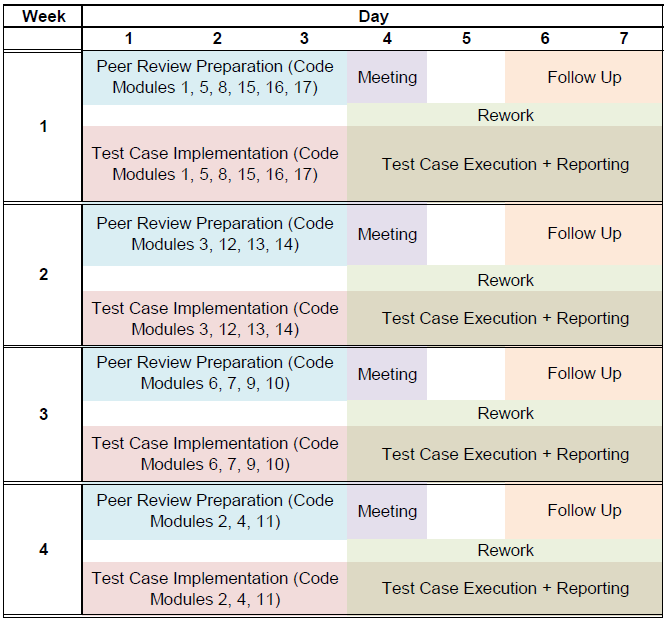
\includegraphics[width=0.9\linewidth]{figures/Implement_Schedule.png}
\end{figure}